\chapter{Axiomas sobre medición de segmentos}

%---------- axioma 2.1
\begin{tcolorbox}[colframe=white]
\begin{axioma}
    A todo par de puntos del plano corresponde un número mayor o igual a cero. Este número es cero si y sólo si los puntos son coincidentes.
\end{axioma}
\end{tcolorbox}

%---------- axioma 2.2
\begin{tcolorbox}[colframe=white]
\begin{axioma}
    Los puntos de una recta pueden ser siempre colocados en correspondencia biunívoca con los números reales, de modo que la diferencia entre esos números sea la distancia entre los puntos correspondientes.
\end{axioma}
\end{tcolorbox}

%---------- axioma 2.3
\begin{tcolorbox}[colframe=white]
\begin{axioma}
   Si el punto $C$ se encuentra entre $A$ y $B$ entonces $$\overline{AB}=\overline{AC} + \overline{CB}$$ 
\end{axioma}
\end{tcolorbox}

    %----------proposición 2.1
    \begin{proposicion}
	Si en una semi-recta $S_{AB}$, tomamos un segmento $AC$ con $\overline{AC}<\overline{AB}$ entonces $C$ está entre $A$ y $B$.\\\\
	    Demostración.-\; Se tiene tres posibilidades:
	    \begin{enumerate}[1.]
		\item $A$ está entre $B$ y $C$, pero no es posible ya que $B,C \in S_{AB}$. 
		\item $B$ está entre $A$ y $C$, pero esto no es posible ya que $\overline{AC}=\overline{AC} + \overline{BC}>\overline{AB}$ contradice a $\overline{AC}<\overline{AB}$.
		\item Por lo tanto, $C$ está entre $A$ y $B$. \\\\
	    \end{enumerate}
    \end{proposicion}

    %----------teorema 2.1
    \begin{teo}
	Sean $A,B,C$ puntos colineales, cuyas coordenadas son $a,b,c \in \mathbb{R}$. El punto $C$ está entre $A$ y $B \Leftrightarrow c$ está entre $a$ y $b$ $(a<c<b$ ó $b<c<a)$\\\\
	    Demostración.-\; Supongamos que $C$ está entre $A$ y $B$ por el axioma 2.3, $\overline{AB} = \overline{AC} + \overline{CB}$, luego $$|a-b| = |c-a| + |b-c| \qquad (1)$$ Si $a<b \quad \Rightarrow \quad b-a = |c-a| + |b-c| \quad \Rightarrow \quad |c-a|<b-a ; \; |b-c|<b-a \quad \Rightarrow \quad c<b ;\; c>a \quad$ y por lo tanto $a<c<b$.\\
	    Por otro lado supongamos que $c$ está entre $a$ y $b$, de donde $|b-a|=|c-b| + |a-c|$ por lo tanto $\overline{AB}=\overline{CB} + \overline{AC}$, así $$\overline{AC}<\overline{AB} \quad 1) \quad y \quad \overline{CB} < \overline{AB} \quad 2)$$
	    Como $C$ está en la recta $AB$ y la recta $AB$ es $S_{AB} \cup S_{BA}$, entonces $C \in S_{AB}$ ó $C\in S_{BA}$. Si $C\in S_{AB}$, de 1) se tiene $C$ entre $A$ y $B$.\\
	    Si $C \in S_{BA}$ de 2) se tiene $\overline{BC}<\overline{BA}$ de donde $C$ está entre $A$ y $B$, por lo tanto, $C$ está entre $A$ y $B$.\\\\
    \end{teo}

%----------definición 2.1
\begin{tcolorbox}[colframe=white]
\begin{def.}
    Llamamos el punto medio del segmento $AB$ a un punto $C$ de este segmento tal que $AC = CB$.
\end{def.}
\end{tcolorbox}

    %----------teorema 2.2.
    \begin{teo}
	Un segmento tiene exactamente un punto medio.\\\\
	    Demostración.-\; (Existencia) Consideremos el segmento $AB$. Sean $a,b$ las coordenadas de $A$ y $B$ respectivamente, de donde claramente vemos que existe $c=\dfrac{a+b}{2}$. Por axioma, existe en la recta $AB$ un punto $C$ cuya coordenada es $c$. Luego por el teorema tenemos que $C$ está entre $A$ y $B$. Además, 
	    $$\overline{AC}=|a-c| = \left| a - \dfrac{a+b}{2}\right| < \left| \dfrac{2a - a -b}{2}\right| = \left| \dfrac{a-b}{2} \right|$$
	    $$\overline{CB} = |c-b| = \left| \dfrac{a+b}{2} - b \right| = \left| \dfrac{a+b-2b}{2} \right| = \left| \dfrac{a-b}{2}\right|$$ de donde $\overline{AC} = \overline{CB}$, así $C$ es el punto medio de $AB$.\\
	    (Unicidad) Sea $C$ el punto obtenido en la primera parte, supongamos $C^{'}$ otro punto medio de $AB$. Luego, $$\overline{AC^{'}} = \overline{BC^{'}} \quad y \quad C^{'} \; está \; estre \; A \; y \;B$$.
	    Luego sean $a,b,c^{'}$ las coordenadas de $A,B,C^{'}$ respectivamente. Tenemos que $c^{'}$ está entre $a$ y $b$.
	    \begin{enumerate}[i)]
		\item Si $a<c^{'}<b \Rightarrow |a-c^{'}|=|b-c^{'}| \quad \Rightarrow \quad c^{'} - a = b - c^{'} \quad \Rightarrow \quad c^{'} = \dfrac{a+b}{2}$
		\item Si $b<c^{'}<a \Rightarrow c^{'}-b=a-^{'} \quad \Rightarrow \quad c^{'} = \dfrac{a+b}{2}$
	    \end{enumerate}
	    Por lo tanto, $c=c^{'}$, luego $C=C^{'}$
    \end{teo}

%----------definición 2.2
\begin{tcolorbox}[colframe=white]
    \begin{def.}
	Sea $A$ un punto del plano y $r>0$. El círculo de centro $A$ y radio $r$ es el conjunto de puntos $B$ tales que $\overline{AB}=r$
    \end{def.}
\end{tcolorbox}

\section{Ejercicios}

\begin{enumerate}[\large \bfseries 1.]

%--------------------1.
    \item Sean $A,B$ y $C$ puntos de una recta. Haga un diseño representándolos, sabiendo que $\overline{AB}=3$, $\overline{AC}=2$ y $\overline{BC}=5$\\\\
    Respuesta.-\;
\begin{center}
    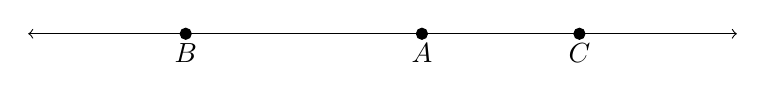
\begin{tikzpicture}
	\draw[<->](-2,0)--(7,0);
	\filldraw[black](3,0) circle(2pt) node[below]{$A$};
	\filldraw[black](0,0) circle(2pt) node[below]{$B$};
	\filldraw[black](5,0) circle(2pt) node[below]{$C$};
    \end{tikzpicture}
\end{center}

    %--------------------2.
    \item Repita el ejercicio anterior, sabiendo que $C$ está entre $A$ y $B$ y que $\overline{AB}=7$ y $\overline{AC}=5.$\\\\
    Respuesta.-\;
\begin{center}
    \begin{tikzpicture}
	\draw[<->](-2,0)--(9,0);
	\filldraw[black](0,0) circle(2pt) node[below]{$A$};
	\filldraw[black](7,0) circle(2pt) node[below]{$B$};
	\filldraw[black](5,0) circle(2pt) node[below]{$C$};
    \end{tikzpicture}
\end{center}

    %--------------------3.
    \item Diseñe una recta y sobre ella marque dos puntos $A$ y $B$. Suponga que la coordenada del punto $A$ sea cero y la del punto $B$ sea $1$. Marque ahora puntos cuyas coordenadas son $3,5,5/2,1/3,3/2,2,-1,-2,-5,-1/3,-5/3$\\\\
    Respuesta.-\;
\begin{center}
    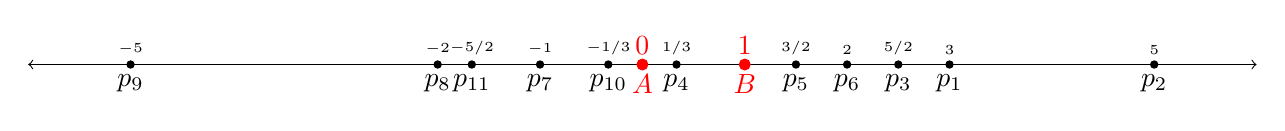
\begin{tikzpicture}[scale=1.3]
	\draw[<->](-6,0)--(6,0);
	\filldraw[red](0,0) circle(1.5pt) node[below]{$A$} node[above]{$0$};
	\filldraw[red](1,0) circle(1.5pt) node[below]{$B$} node[above]{$1$};
	\filldraw[black](3,0) circle(1pt) node[below]{$p_1$} node[above]{\tiny$3$};
	\filldraw[black](5,0) circle(1pt) node[below]{$p_2$} node[above]{\tiny$5$};
	\filldraw[black](5/2,0) circle(1pt) node[below]{$p_3$} node[above]{\tiny$5/2$};
	\filldraw[black](1/3,0) circle(1pt) node[below]{$p_4$} node[above]{\tiny$1/3$};
	\filldraw[black](3/2,0) circle(1pt) node[below]{$p_5$} node[above]{\tiny$3/2$};
	\filldraw[black](2,0) circle(1pt) node[below]{$p_6$} node[above]{\tiny$2$};
	\filldraw[black](-1,0) circle(1pt) node[below]{$p_7$} node[above]{\tiny$-1$};
	\filldraw[black](-2,0) circle(1pt) node[below]{$p_8$} node[above]{\tiny$-2$};
	\filldraw[black](-5,0) circle(1pt) node[below]{$p_9$} node[above]{\tiny$-5$};
	\filldraw[black](-1/3,0) circle(1pt) node[below]{$p_{10}$} node[above]{\tiny$-1/3$};
	\filldraw[black](-5/3,0) circle(1pt) node[below]{$p_{11}$}  node[above]{\tiny$-5/2$};
    \end{tikzpicture}
\end{center}

    %--------------------4.
    \item Sean $A_1$ y $A_2$ puntos de coordenadas $1$ y $2$. De la coordenada del punto medio $A_3$ del segmento $A_1 A_2$. De la coordenada del punto medio $A_4$ del segmento $A_2A_3$. De la coordenada del punto medio $A_5$ del segmento $A_3A_4$.\\\\
    Respuesta.-\; Dado que $A_3$ es el punto medio del segmento $A_1 A_2$, la coordenada $A_3$ será la media aritmética.
    $$A_3=\dfrac{A_1 + A_2}{2}=\dfrac{1+2}{2}=\dfrac{3}{2}$$
    Luego calculamos análogamente para los otros puntos.
    $$A_4=\dfrac{\dfrac{3}{2}+2}{2}=\dfrac{7}{4}$$
    $$A_5=\dfrac{\dfrac{3}{2}+\dfrac{7}{4}}{2}=\dfrac{13}{8}$$\\\\

    %--------------------5.
    \item Sean $a,b,c,d$ números reales distintos de cero. Pruebe que, si $\dfrac{a}{b}=\dfrac{c}{d}$ entonces
    \begin{enumerate}[\bfseries a)]
	%----------a)
	\item $\dfrac{a}{c}=\dfrac{b}{d}$ y $\dfrac{d}{b}=\dfrac{c}{a}$\\\\
	Demostración.-\; Sea $\dfrac{a}{b}=\dfrac{c}{d}$ entonces por hipótesis $\dfrac{a}{b}\cdot \dfrac{b}{c}=\dfrac{c}{d} \cdot \dfrac{b}{c}$ luego $\dfrac{a}{c}=\dfrac{b}{d}$\\\\ 

	%----------b)
	\item $\dfrac{a+c}{a}=\dfrac{c+d}{c}$ y $\dfrac{a-c}{a}=\dfrac{c-d}{c}$\\\\
	Demostración.-\; Sea $\dfrac{a}{b}=\dfrac{c}{d}$ entonces $\dfrac{db}{ac}\cdot \dfrac{a}{b}$ luego $1+\dfrac{d}{c}=1+\dfrac{b}{a}$, de donde $\dfrac{c}{c}\cdot \dfrac{d}{c}=\dfrac{a}{a}\cdot \dfrac{b}{a}$ y por lo tanto $\dfrac{c+d}{c}=\dfrac{b+a}{a}$\\\\

	%----------c)
	\item $\dfrac{a+b}{b}=\dfrac{c+d}{d}$ y $\dfrac{a-b}{b}=\dfrac{c-d}{d}$\\\\
	Demostración.-\; Sea $\dfrac{a}{b}=\dfrac{c}{d}$ entonces $\dfrac{a}{b}\cdot \dfrac{bd}{ac}=\dfrac{c}{d}\cdot \dfrac{db}{ac}$ luego similar al ejercicio anterior tenemos $-1 \cdot \dfrac{d}{c}=-1 \cdot \dfrac{b}{a}$ y por lo tanto $\dfrac{c-d}{c}=\dfrac{a-b}{a}$\\\\

    \end{enumerate}

    %-------------------6.
    \item Si $P$ es el punto de intersección de los círculos de radio $r$ y centros en $A$ y $B$, muestre que $\overline{PA}=\overline{PB}$\\\\
    \begin{center}
	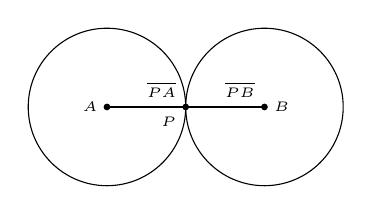
\begin{tikzpicture}
	    \draw(0,0) circle(1cm);
	    \draw(2,0) circle(1cm);
	    \filldraw[black](1,0) circle(1pt) node[below left]{\tiny$P$};
	    \filldraw[black](0,0) circle(1pt) node[left]{\tiny$A$};
	    \filldraw[black](2,0) circle(1pt) node[ right]{\tiny$B$};
	    \draw(0,0)--(1,0)node[above left ]{\tiny$\overline{PA}$};
	    \draw(1,0)--(2,0)node[above left]{\tiny$\overline{PB}$};
	\end{tikzpicture}
    \end{center}
    Demostración.-\; Como el punto $P$ está en la intersección de los dos círculos. Entonces $P$ pertenece al círculo con centro $A$ y radio $r$, y por definición de círculo, $PA = r$, igualmente $P$ pertenece al círculo con centro $B$ y radio $r$, por definición de círculo, $PB = r$, lo que implica que $PA = PB$.\\\\

    %--------------------7.
    \item Usando regla y compás (regla no numerada), describa un método para la construcción de un triángulo con dos lados de misma longitud. (Un triángulo así, es llamado triángulo isósceles).\\\\
    Respuesta.-\; Considere un segmento $AB$. Con un compás centrada en $A$, dibuja una circunferencia de radio $AB$. Ahora con el centro en $B$, dibuja un círculo de radio $BA$. La intersección entre los dos círculos generará los puntos $C$ y $D$. Haciendo el triángulo $CAD$ tendremos un triángulo isósceles con base $CD$ y lados $CA,AD$.
    \begin{center}
	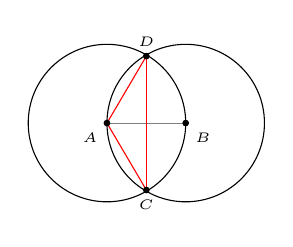
\begin{tikzpicture}
	    \draw[gray](0,0)--(1,0);
	    \draw[red](0,0)--(0.5,.85);
	    \draw[red](0,0)--(.5,-.85);
	    \draw[red](.5,-.85)--(.5,.85);
	    \draw(0,0) circle(1cm);
	    \filldraw[black](0,0) circle(1pt) node[below left]{\tiny$A$};
	    \draw(1,0) circle(1cm);
	    \filldraw[black](1,0) circle(1pt) node[below right]{\tiny$B$};
	    \filldraw[black](0.5,.85) circle(1pt) node[above]{\tiny$D$};
	    \filldraw[black](0.5,-.85) circle(1pt) node[below]{\tiny$C$};

	\end{tikzpicture}
    \end{center}

    %--------------------8.
    \item Describa un método para construir un triángulo con sus tres lado de misma longitud.( Un triángulo así, es llamado triángulo equilátero ).\\\\
    Respuesta.-\; Se traza una recta y se marca dos puntos $A$ y $B$ en ella. Con el centro en $A$ y luego en $B$, se generan dos circunferencias de radio $r$ generando el punto $C$, después trazamos los segmentos $AC, AB$ y $BC$ que generará $\triangle ABC$ con lados iguales a $r$.
    \begin{center}
	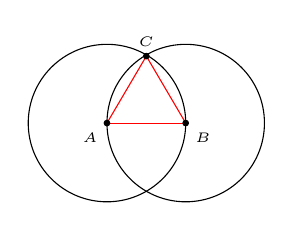
\begin{tikzpicture}
	    \draw[red](0,0)--(1,0);
	    \draw[red](0,0)--(0.5,.85);
	    \draw[red](1,0)--(.5,.85);
	    \draw(0,0) circle(1cm);
	    \filldraw[black](0,0) circle(1pt) node[below left]{\tiny$A$};
	    \draw(1,0) circle(1cm);
	    \filldraw[black](1,0) circle(1pt) node[below right]{\tiny$B$};
	    \filldraw[black](0.5,.85) circle(1pt) node[above]{\tiny$C$};
	\end{tikzpicture}
    \end{center}

    %--------------------9.
    \item Muestre que, si $a<b$ entonces $a<\dfrac{a+b}{2}$ y $b>\dfrac{a+b}{2}$\\\\
    Demostración.-\; Daremos una demostración que va mas allá del ejercicio en si planteado para entender de mejor manera esta proposición.\\\\
    Demostrar que si $0<a < b$, entonces $$a<\sqrt{ab}<\dfrac{a+b}{2} < b$$\\
    \begin{enumerate}[1.]
	\item $a<\sqrt{ab}$\\\\
Si \; $4a<b$ entonces $a^2<ab$ y por raíz cuadrada dado que $a,\;b>0$ entonces $a<\sqrt{ab}$\\
	\item $\sqrt{ab}<\dfrac{a+b}{2}$\\\\
En vista de que $a, \; b > 0$ y $a<b$ entonces $a-b>0$, \; $(a-b)^2>0$ por lo tanto, $a^2-2ab+b^2>0 \Rightarrow 2ab< a^2+b^2 \Rightarrow 2ab-2ab+2ab<a^2+b^2 \Rightarrow 4ab < a^2+2ab +b^2 \Rightarrow 4ab < (a+b^)2 \Rightarrow ab < \displaystyle \left( \frac{a+b}{2} \right) ^2 \Rightarrow \sqrt{ab}<\frac{a+b}{2} $ \\
	\item $\displaystyle\frac{a+b}{2}<b$\\\\
Si $a<b$ entonces $a+b<2b$ por lo tanto $\displaystyle\frac{a+b}{2}<b$\\\\
    \end{enumerate}

    %--------------------10.
    \item ¿Es posible construir un triángulo con lados de longitud $3,8$ y $5$?\\\\
    Respuesta.-\; No, ya que la desigualdad triangular establece que la suma de dos lados cualesquiera de un triángulo es mayor que el tercer lado, es decir, si tomamos las medidas de los lados $5$ y $3$, tendremos $8$ que será igual a la tercera medida.\\\\

    %--------------------11.
    \item El círculo de radio $r_1$ centrado en $A$ intersecta al círculo de radio $r_2$ centrado en $B$ en exactamente dos puntos. ¿Qué se puede afirmar sobre $\overline{AB}$?\\\\
    Respuesta.-\; Considere el círculo de radio $r_2$ con centro en $A$ y el círculo de radio $r_1$ con centro en $B$ y cuyo segmento $AB$ forma los puntos $C$ y $D$. Note que $AB = AD + CB - CD$ y también que $AD = r_2, CB = r_1$ y que $CD$ es un segmento no nulo. Luego observe que  $AB = r_2 + r_1 - CD$, lo que implica que $AB <r_2 + r_1$\\
    \begin{center}
	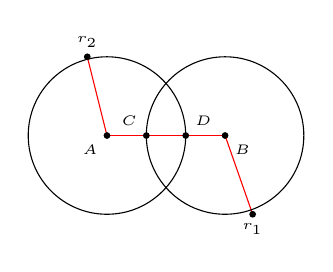
\begin{tikzpicture}
	    \draw[red](-.25,0)--(1.25,0);
	    \draw[red](-.25,0)--(-.5,1);
	    \draw[red](1.25,0)--(1.6,-1);
	    \draw(-.25,0) circle(1cm);
	    \draw(1.25,0) circle(1cm);
	    \filldraw[black](-.25,0) circle(1pt) node[below left]{\tiny$A$};
	    \filldraw[black](1.25,0) circle(1pt) node[below right]{\tiny$B$};
	    \filldraw[black](0.25,0) circle(1pt) node[above left]{\tiny$C$};
	    \filldraw[black](0.75,0) circle(1pt) node[above right]{\tiny$D$};
	    \filldraw[black](1.6,-1) circle(1pt) node[below]{\tiny$r_1$};
	    \filldraw[black](-.5,1) circle(1pt) node[above]{\tiny$r_2$};
	\end{tikzpicture}
    \end{center}

    %--------------------12.
    \item Considere un círculo de radio $r$ y centro $A$. Sean $B$ y $C$ puntos de este círculo. ¿Qué se puede afirmar sobre el triángulo $ABC$?\\\\
    \begin{center}
	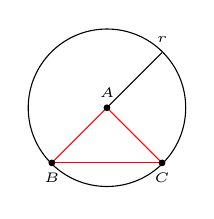
\begin{tikzpicture}
	    \draw(0,0)--(.7,.7)node[above]{\tiny$r$};
	    \draw[red](0,0)--(-.7,-.7);
	    \draw[red](0,0)--(.7,-.7);
	    \draw[red](-.7,-.7)--(.7,-.7);
	    \draw(0,0) circle(1cm);
	    \filldraw[black](0,0) circle(1pt) node[above]{\tiny$A$};
	    \filldraw[black](-.7,-.7) circle(1pt) node[below]{\tiny$B$};
	    \filldraw[black](.7,-.7) circle(1pt) node[below]{\tiny$C$};
	\end{tikzpicture}
    \end{center}
    Respuesta.-\; Si los puntos $B$ y $C$ pertenecen a la circunferencia que forma el círculo entonces $AB = AC = r$ por lo tanto el triángulo es isósceles con base $AB$.\\\\

    %--------------------13.
    \item Considere un círculo de radio $r$ y centro $O$. Sea $A$ un punto de este círculo y sea $B$ un punto tal que el triángulo $OAB$ es equilátero. ¿Cuál es la posición del punto $B$ en relación al círculo?\\\\
    Respuesta.-\; Dado que el triángulo es equilátero y uno de sus lados es el segmento $OA$ de tamaño $r$, entonces $OB = r$, luego el punto $B$ está a una distancia $r$ del centro del círculo, es decir, $B$ pertenece a la circunferencia.\\\\

    %--------------------14.
    \item Dos círculos de mismo radio y centro $A$ y $B$ se intersectan en dos puntos $C$ y $D$. ¿Qué se puede afirmar sobre los triángulos $ABC$ y $ACD$? ¿Y, sobre el cuadrilátero $ACBD$?\\\\
    Respuesta.-\; 
    \begin{center}
	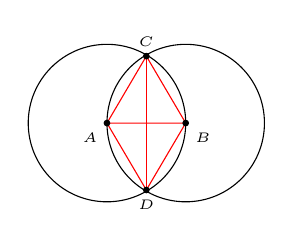
\begin{tikzpicture}
	    \draw[red](0,0)--(.5,.85)--(1,0)--(.5,-.85)--(0,0)--(1,0);
	    \draw[red](.5,.85)--(.5,-.85);
	    \draw(0,0) circle(1cm);
	    \draw(1,0) circle(1cm);
	    \filldraw[black](0,0) circle(1pt) node[below left]{\tiny$A$};
	    \filldraw[black](1,0) circle(1pt) node[below right]{\tiny$B$};
	    \filldraw[black](.5,.85) circle(1pt) node[above]{\tiny$C$};
	    \filldraw[black](.5,-.85) circle(1pt) node[below]{\tiny$D$};
	\end{tikzpicture}
    \end{center}
    Los triángulos $ABC$ y $ACD$ son isósceles porque $AC, BC = r $ y $AD = r$  así también $BD = r$. Como el paralelogramo ACBD está formado por la unión de $\triangle ABC$ y $\triangle ADB$, sus lados serían los segmentos que forman el triángulo,  luego $AC = BC = AD = BD = r$. Entonces el polígono es un cuadrilátero de lados iguales y los triángulos son isósceles.\\\\

    %--------------------15.
    \item Dado un segmento $AB$ muestre que existe y es único, un punto $C$ entre $A$ y $B$ tal que $$\dfrac{\overline{AC}}{\overline{BC}}=a,$$ donde $a$ es cualquier número real positivo.\\\\
    Demostración.-\; Sean $x, b$ y $c$ las coordenadas de los puntos $A, B$ y $C$. Podemos suponer que $a <b <c$. Luego para el caso de $x> b> c$, se resuelve de forma totalmente análoga. Entonces, por el axioma $III_2$ el problema a demostrar pasa por la existencia de un solo punto $B$ entre $A$ y $C$ tal que $\dfrac{m(AC)}{m(BC)}=a$, equivale a mostrar que existe un único número real $b$ tal que $x<b<c$ y $\dfrac{b-x}{c-b}=a$.\\
    Resolviendo en $b$ obtenemos que la única solución es $b=\dfrac{x+ca}{1+a}$. Finalmente, queda demostrar que este $b$ encontrado satisfaga a $x<b<c$. Es decir,
    $$x=\dfrac{x+ax}{1+a}<\dfrac{x+ca}{1+a}<\dfrac{c+ca}{1+a}$$
    La unicidad del punto $B$ también es una consecuencia del axioma $III_2$.\\\\

    %--------------------16.
    \item Pruebe que un segmento de recta que une un punto del círculo, con un punto dentro del mismo, tiene un punto en común con el círculo.\\\\
    Demostración.-\; Sea $C$ cualquier punto fuera de un círculo de centro $O$, entonces $OC> r$ donde $r$ es el radio del círculo. Entonces, hay un punto $D \in OC$ tal que $\overline{OD} = r$. Dado que el círculo está formado por todos los puntos en el plano que están a una distancia $r$ del punto $O$, entonces el punto $D$ pertenece a la intersección del segmento $OC$ con la circunferencia.\\\\

    %--------------------17.
    \item Dados los puntos $A$ y $B$ y un número real $r$ mayor que $\overline{AB}$, el conjunto de los puntos $C$ que satisfacen $\overline{CA}+\overline{CB}=r$ es llamado elipse. Establezca los conceptos de región interior y de región exterior a un elipse.\\\\
    Respuesta.-\; Si $\overline{CA} + \overline{CB}> r$, entonces el conjunto de puntos es externo. Si $\overline{CA} + \overline{CB} <r$, entonces el conjunto de puntos será interno.\\\\

    %--------------------18.
    \item Un conjunto $M$ de puntos del plano es acotado si existe un círculo $C$ tal que todos los puntos de $M$ están dentro de $C$. Pruebe que cualquier conjunto finito de puntos es acotado. Pruebe también que los segmentos son acotados. Concluya el mismo resultado para los triángulos.\\\\
    Demostración.-\; Dado el conjunto de puntos $P_1, P_2, ..., P_n$ tome un solo punto $P_i$ que usaremos para el centro de la circunferencia, para cada punto $P_j$ con $i\neq j$ y $j$ variando de $1$ a $n$ quitando el propio $i$, pasará a un segmento diferente. Deje que $P_i P_j$ sea el más grande de todos los segmentos, por lo que se marca a sí mismo un punto $Q (P_1 - P_j - Q)$ en la línea que pasa por el segmento de modo que por $P_1 Q$ definimos un círculo de radio $r = P_1 Q$ que contendrá todos los demás, ya que el segmento que establece su radio con relación al centro $P_1$ es mayor que los demás definidos por todos los demás puntos.\\\\

    %--------------------19.
    \item Pruebe que la unión de una cantidad finita de conjuntos acotados es también un conjunto acotado.\\\\
    Demostración.-\;

    %--------------------20.
    \item Muestre que dado un punto $P$ y un conjunto acotado $M$, existe un círculo $C$ con centro en $P$ tal que todos los puntos de $M$ están dentro de $C.$\\\\
    Demostración.-\;

    %--------------------21.
    \item Pruebe que las rectas son conjuntos no acotados.\\\\
    Demostración.-\; Supongamos que las rectas son conjuntos acotados, pero por el axioma 1.2 esta proposición es absurda ya que la recta real consta de infinitos puntos. Por lo tanto las rectas son conjuntos no acotados.\\\\

\end{enumerate}
